\documentclass[border=6pt]{standalone}
\usepackage{tikz}
\usepackage[edges]{forest}
\usetikzlibrary{arrows.meta,positioning,calc,decorations.pathreplacing,shapes.geometric}
\begin{document}
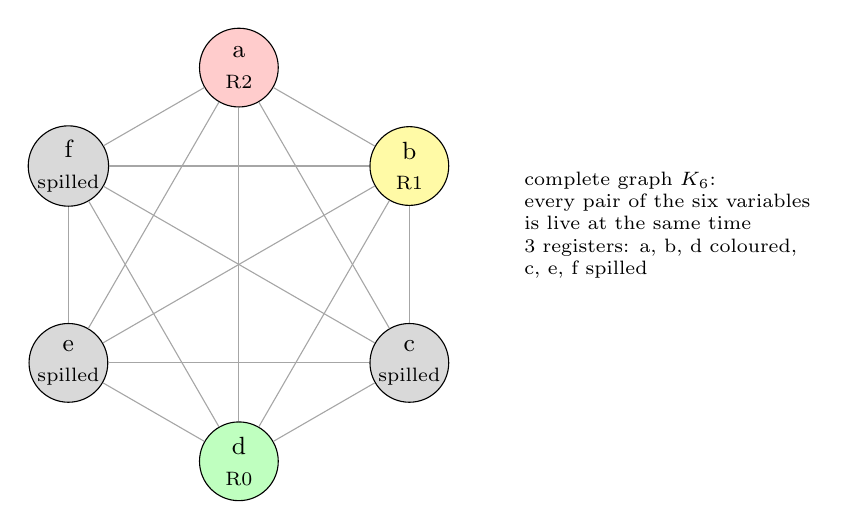
\begin{tikzpicture}[font=\small,v/.style={draw,circle,minimum size=1.0cm,inner sep=0pt,align=center}]
\node[v,fill=red!20] (a) at (0.000,2.500) {a\\{\scriptsize R2}};
\node[v,fill=yellow!35] (b) at (2.165,1.250) {b\\{\scriptsize R1}};
\node[v,fill=gray!30] (c) at (2.165,-1.250) {c\\{\scriptsize spilled}};
\node[v,fill=green!25] (d) at (0.000,-2.500) {d\\{\scriptsize R0}};
\node[v,fill=gray!30] (e) at (-2.165,-1.250) {e\\{\scriptsize spilled}};
\node[v,fill=gray!30] (f) at (-2.165,1.250) {f\\{\scriptsize spilled}};
\draw[gray!70] (a)--(b);
\draw[gray!70] (a)--(c);
\draw[gray!70] (a)--(d);
\draw[gray!70] (a)--(e);
\draw[gray!70] (a)--(f);
\draw[gray!70] (b)--(c);
\draw[gray!70] (b)--(d);
\draw[gray!70] (b)--(e);
\draw[gray!70] (b)--(f);
\draw[gray!70] (c)--(d);
\draw[gray!70] (c)--(e);
\draw[gray!70] (c)--(f);
\draw[gray!70] (d)--(e);
\draw[gray!70] (d)--(f);
\draw[gray!70] (e)--(f);
\node[font=\scriptsize,anchor=west,align=left] at (3.5,0.5) {complete graph $K_6$:\\every pair of the six variables\\is live at the same time\\3 registers: a, b, d coloured,\\c, e, f spilled};
\end{tikzpicture}
\end{document}
